% ======================================================================
% 深圳大学实验报告模板（SZU Experiment Report Template）
% 项目一：基于 NumPy 的 OpenCLIP ViT-B-32 图像编码器复现
% 编译方式：XeLaTeX
% ======================================================================
\documentclass[a4paper,12pt]{article}
% ---------- 中文与字体支持（修复xeCJK警告，Overleaf稳定版） ----------
\usepackage{fontspec}
\usepackage{xeCJK}
\setCJKmainfont{Noto Sans CJK SC}[
    BoldFont={Noto Sans CJK SC Bold}
]
\setmainfont{Latin Modern Roman}
% ---------- 页面设置与常用宏包 ----------
\usepackage{geometry}
\geometry{left=1in, right=1in, top=1in, bottom=1in}
\usepackage{longtable}
\usepackage{graphicx}
\usepackage{fancyhdr}
% \usepackage{tikz}
% \usetikzlibrary{calc}   % 暂时注释，避免除以0报错
\usepackage{verbatim}
\usepackage{float}
\usepackage{booktabs}
\usepackage{amsmath}
\usepackage{amssymb}
\usepackage{xcolor}
% ---------- 页眉页脚设置 ----------
\pagestyle{fancy}
\fancyhf{}
\fancyhead[C]{}
\fancyhead[R]{}
\renewcommand{\headrulewidth}{0.4pt}
\renewcommand{\footrulewidth}{0pt}
% ---------- 自定义命令（可选） ----------
\newcommand{\code}[1]{\texttt{#1}}
\newcommand{\todo}[1]{\textbf{\color{red}[TODO: #1]}}
% ======================================================================
\begin{document}
% ============================================================
% 封面页
% ============================================================
\begin{titlepage}
    \centering
    \vspace*{2cm}
    \Huge{\textbf{深 \ 圳 \ 大 \ 学 \ 实 \ 验  \ 报 \ 告}}\\[1.5cm]
    {\Large
    \renewcommand{\arraystretch}{1.55}
    \begin{tabular}{@{}r@{\hspace{0.9cm}}l@{}}
    \textbf{课程名称} & \underline{Python 程序设计} \\[0.25cm]
    \textbf{项目名称} & \underline{基于 NumPy 的图像特征提取编码器复现} \\[0.25cm]
    \textbf{学 \quad 院} & \underline{人工智能学院} \\[0.25cm]
    \textbf{专 \quad 业} & \underline{人工智能IEEE荣誉班} \\[0.25cm]
    \textbf{指导教师} & \underline{舒婷} \\[0.25cm]
    \textbf{报 \ 告 \ 人} & \underline{贺康博}\hspace{0.5cm}\textbf{学号}\hspace{0.4cm}\underline{2025681113} \\[0.25cm]
    \textbf{实验时间} & \underline{2026.11.19} \\[0.25cm]
    \textbf{提交时间} & \underline{2026.11.24} \\
    \end{tabular}}
    \\[1.5cm]
    \vfill
    \Large{\textbf{教务处制}}
\end{titlepage}

\newpage
% ============================================================
% 正文部分
% ============================================================
\section{Objectives（实验目标）}
本项目的目标是：在不进行模型训练、不依赖 PyTorch 或 GPU 的前提下，仅使用
NumPy 完成 OpenCLIP ViT-B-32 图像塔（image encoder）的前向计算，从输入图像中
提取数值特征。给定预处理后的图像批次与已训练好的模型参数 $\theta$，程序需要为
每张图像输出一个 512 维、长度为 1 的浮点向量，作为后续图像检索、图文匹配等任务
使用的图像特征。
具体要求包括：
\begin{enumerate}
    \item 补全 \texttt{image\_encoder.py} 中 TODO-01 到 TODO-06 共六组代码；
    \item 输出在形状、数据类型（float32）、数值上与课程提供的独立 FP32 参考对齐；
    \item 代码结构保持与最终项目中 \texttt{ImageEncoder} 的接口一致，方便之后复用。
\end{enumerate}
\section{Overview（方案概览）}
整体流程与标准 ViT 图像编码器一致，如图~\ref{fig:vit-arch} 所示。输入图像先经过
课程提供的预处理（缩放、中心裁剪到 $224\times224$、按通道均值方差归一化），随后
进入本次实现的编码器：
\begin{enumerate}
    \item[Spot 1] \textbf{切分 Patch}：把 $224\times224$ 的 RGB 图像按 $32\times32$
          切成 $7\times7=49$ 个 patch，每个 patch 按通道、高、宽展平为 3072 维向量；
    \item[Spot 2] \textbf{嵌入编码}：patch 经线性投影到 768 维，拼上可学习的 CLS
          标记并加上位置编码，得到 50 个 token；
    \item[Spot 3] \textbf{Transformer 堆叠}：12 个结构相同的 Block 依次做多头自注意力
          和 MLP，每个 Block 包含两次残差连接；最后取 CLS token，经过 LayerNorm、
          512 维投影和单位长度归一化，得到最终图像特征。
\end{enumerate}
模型固定规格为：输入 $224\times224$，patch 大小 32，宽度 768，12 个注意力头，
每个头 64 维，共 12 层，MLP 中间宽度 3072，输出维度 512。
\begin{figure}[t]
    \centering
    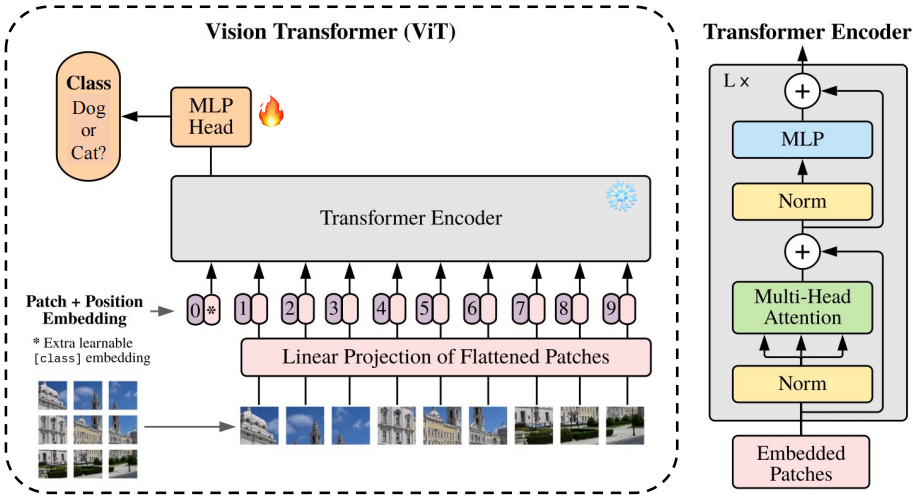
\includegraphics[width=0.92\linewidth]{figs/vit_overview.png}
    \caption{Vision Transformer 整体结构：Patch 与位置嵌入、Transformer 编码器、CLS 输出头（图为课程课件示意图）。}
    \label{fig:vit-arch}
\end{figure}
\section{Implementations（实现要点）}
本次只修改 \texttt{image\_encoder.py}，辅助函数（LayerNorm、GELU、注意力系数、
单位向量）和图像预处理均由课程提供。六组 TODO 的实现要点如下。
\subsection{Patch 切分（TODO-01）}
输入形状为 $[B,3,224,224]$。先用 \texttt{reshape} 把空间维度拆成网格轴和 patch
轴，再用 \texttt{transpose} 调整轴顺序，使 patch 按“从左到右、从上到下”的顺序
排列，patch 内部按 C、H、W 展平，最终得到 $[B,49,3072]$：
\begin{verbatim}
patches = images.reshape(B, C, gh, patch, gw, patch)
patches = patches.transpose(0, 2, 4, 1, 3, 5)
return patches.reshape(B, gh * gw, C * patch * patch)
\end{verbatim}
\subsection{多头注意力（TODO-02、TODO-03）}
\texttt{split\_heads} 把特征轴拆成“头数 $\times$ 头维度”，并把头轴移到 token 轴
之前：$[B,N,768]\rightarrow[B,12,N,64]$。注意力打分时，Q 与转置最后两个轴的 K
做矩阵乘，并除以 $\sqrt{\text{head\_dim}}$：
\begin{verbatim}
scores = (q @ k.transpose(0, 1, 3, 2)) / sqrt(head_dim)
coefficients = attention_weights(scores)   # softmax，课程提供
context = coefficients @ v
merged = context.transpose(0, 2, 1, 3).reshape(B, N, width)
return merged @ out_weight.T + out_bias
\end{verbatim}
注意力/MLP 的线性权重按 $[\text{out},\text{in}]$ 存储，因此计算时需要转置；
最后的输出投影同样使用 \texttt{out\_weight.T}。
\subsection{Transformer Block（TODO-04）}
每个 Block 有两条残差路径。先对输入做 LayerNorm 再算注意力，把注意力更新加回
原始输入；第二次 LayerNorm 后的结果进入 MLP（GELU 激活），再把 MLP 更新加回第一次
残差的结果：
\begin{verbatim}
update  = attention(norm1(x), causal=causal)
residual = x + update
u       = norm2(residual)
hidden  = gelu(u @ fc1_weight.T + fc1_bias)
mlp_update = hidden @ fc2_weight.T + fc2_bias
return residual + mlp_update
\end{verbatim}
\subsection{嵌入与输出头（TODO-05、TODO-06）}
Patch 投影没有偏置；投影后在 token 轴开头拼接 CLS 标记，再加上可学习位置编码。
最终输出时只取序列第 0 行（CLS token），经过 post-LayerNorm 和投影矩阵得到 512
维向量。注意 \texttt{visual.proj} 已经是 $[\text{in},\text{out}]$ 布局，不再转置；
最后由课程提供的 \texttt{unit\_vector} 按行归一化到单位长度。
\begin{verbatim}
projected = patches @ patch_weight.T
tokens    = concatenate([cls, projected], axis=1) + position
cls_token = tokens[:, 0, :]
output    = post_norm(cls_token) @ projection
return unit_vector(output)
\end{verbatim}
\section{Results（结果与证据）}
\subsection{环境与复现步骤}
运行环境为 Python 3.13、NumPy 2.5.5、Pillow 12.3，无需 GPU、PyTorch 或网络。
在项目根目录下依次执行：
\begin{verbatim}
python -m pip install -r requirements.txt
python check.py --stage all
python run.py --output output_tokens.npz
\end{verbatim}
\subsection{分阶段数值校验}
\texttt{check.py} 将本程序的中间结果与独立 FP32 参考逐阶段比较，输出最大绝对误差
和平均绝对误差。各阶段实际结果如表~\ref{tab:stage-err}，全部通过对应容差
（内部 token：atol $2\times10^{-4}$；输出与 batch：atol $2\times10^{-5}$，
rtol $2\times10^{-4}$）。
\begin{table}[H]
    \centering
    \caption{分阶段数值误差（课程参考为独立 FP32 前向结果）}
    \label{tab:stage-err}
    \begin{tabular}{lclcc}
        \toprule
        阶段 & 输出形状 & 最大绝对误差 & 平均绝对误差 & 结论 \\
        \midrule
        preprocess  & $(10,3,224,224)$ & $0.000\mathrm{e}{+}00$ & $0.000\mathrm{e}{+}00$ & PASS \\
        patches     & $(2,49,3072)$    & $0.000\mathrm{e}{+}00$ & $0.000\mathrm{e}{+}00$ & PASS \\
        tokens      & $(2,50,768)$     & $4.005\mathrm{e}{-}05$  & $1.289\mathrm{e}{-}06$ & PASS \\
        block0      & $(2,50,768)$     & $7.063\mathrm{e}{-}06$  & $3.250\mathrm{e}{-}07$ & PASS \\
        last\_tokens& $(2,50,768)$     & $4.768\mathrm{e}{-}05$  & $2.696\mathrm{e}{-}06$ & PASS \\
        output      & $(10,512)$       & $5.439\mathrm{e}{-}07$  & $8.311\mathrm{e}{-}08$ & PASS \\
        batch       & $(3,512)$        & $4.619\mathrm{e}{-}07$  & $7.632\mathrm{e}{-}08$ & PASS \\
        \bottomrule
    \end{tabular}
\end{table}
\subsection{输出核验}
对课程提供的 10 张本地图片运行 \texttt{run.py}，得到形状 $(10,512)$ 的 float32
数组，所有数值均有限；每行特征的 L2 范数均为 $1.0$，符合单位长度要求。与参考输出
逐张计算余弦相似度，范围为 $0.9999998\sim1.0000001$。
\texttt{batch} 阶段还对图片顺序做了打乱并加入重复图片，输出仍与参考一致，说明实现
不依赖固定输入顺序。10 张图片两两之间的余弦相似度在 $0.4624\sim0.6739$ 之间，
相似度最高的一对是 \texttt{image\_01} 与 \texttt{image\_10}（0.6739），两张图都
属于艺术展览/博物馆场景，特征上更接近，结果符合直观。
\section{Discussion（分析与反思）}
\subsection{一个形状变化：多头拆分与合并}
实现中最容易出错的是注意力头的轴组织。拆分时先把 $[B,N,768]$ 按最后一维 reshape
成 $[B,N,12,64]$，再 transpose 成 $[B,12,N,64]$；合并时要沿相反方向做
transpose 和 reshape。如果 reshape 后直接把头轴留在 token 轴之后，打分矩阵的形状
虽然可能看不出明显报错，但每个头看到的特征会被打乱，后续阶段误差会逐层放大。
对照教学小例子和参考形状逐阶段检查后，才确认轴顺序是正确的。
\subsection{修复的一个 Bug：K 的转置范围与权重布局}
调试过程中修复的主要问题是：真实模型的 K 是 4 维数组 $[B,H,N,64]$，打分时只能
交换最后两个轴（\texttt{k.transpose(0,1,3,2)}），不能直接写成教学二维例子里的
\texttt{k.T}，否则 batch 轴和头轴也会被一起转置，导致分数完全错乱。另一个容易混淆
的点是权重布局：注意力和 MLP 的线性权重是 $[\text{out},\text{in}]$，需要取
\texttt{.T}；而最终投影 \texttt{visual.proj} 已经是 $[\text{in},\text{out}]$，
不能再转置。这两处方向在代码注释和检查阶段都做了核对。
\subsection{局限与改进方向}
本项目只复现图像塔的前向计算，不涉及参数训练；GELU 按课程提供的方式用 Python
循环逐元素计算，图片批次较大时速度偏慢，后续可以改用向量化实现。目前测试覆盖课程
提供的 10 张图片以及打乱/重复 batch，之后还可以加入更多尺寸、更多类别的图片做稳健性
检查。代码保留了可选的因果掩码开关和与最终项目一致的类接口，方便之后把同一套
Transformer 代码复用到文本编码器。
\subsection{本人贡献与使用帮助}
本人独立完成了 \texttt{image\_encoder.py} 中六组 TODO 的编写与调试验证；
\texttt{helpers.py}、图像预处理、参数加载与数值校验脚本由课程提供。实现过程中参考
了课件第 46--70 页的计算公式，以及 \texttt{transformer\_steps.py} 中的微型
Transformer 演算；参考输出文件只用于 \texttt{check.py} 比对，没有作为编码器输入。
\newpage
\vspace{1cm}

\noindent \textbf{指导教师批阅意见：}
\vspace{5.5cm}

\noindent \textbf{成绩评定：}
\vspace{2.2cm}

\begin{flushright}
\textbf{指导教师签字：}\;\underline{\hspace{3.6cm}}\\[0.15cm]
\vspace{0.55cm}
\textbf{年}\;\underline{\hspace{1.4cm}}\quad
\textbf{月}\;\underline{\hspace{1.4cm}}\quad
\textbf{日}\;\underline{\hspace{1.4cm}}
\end{flushright}

\vspace{1.2cm}

\noindent \textbf{备注：}

\vspace{0.2cm}

\noindent{\small
注：\;1、报告内的项目或内容设置，可根据实际情况加以调整和补充。

\vspace{0.15cm}

\noindent\hspace*{2.1em}2、教师批改学生实验报告时间应在学生提交实验报告时间后 10 日内。}

\end{document}
